\section{Auswertung}
\label{sec:Auswertung}
Mittelwert der Federkonstanten $\symup{D} = \frac{\symup{F}}{\symup{\triangle x}}$ für $n = 10$ Messdaten ist 
\begin{equation}
\langle \symup{D} \rangle = \frac{1}{n} \sum_{i=1}^n \symup{D_i} = \SI{0.029}{\newton\per\centi\meter}.
\end{equation}
Für diese Rechnung wurde kein Programm, lediglich ein Taschenrechner verwendet.

\begin{figure}
    \centering
    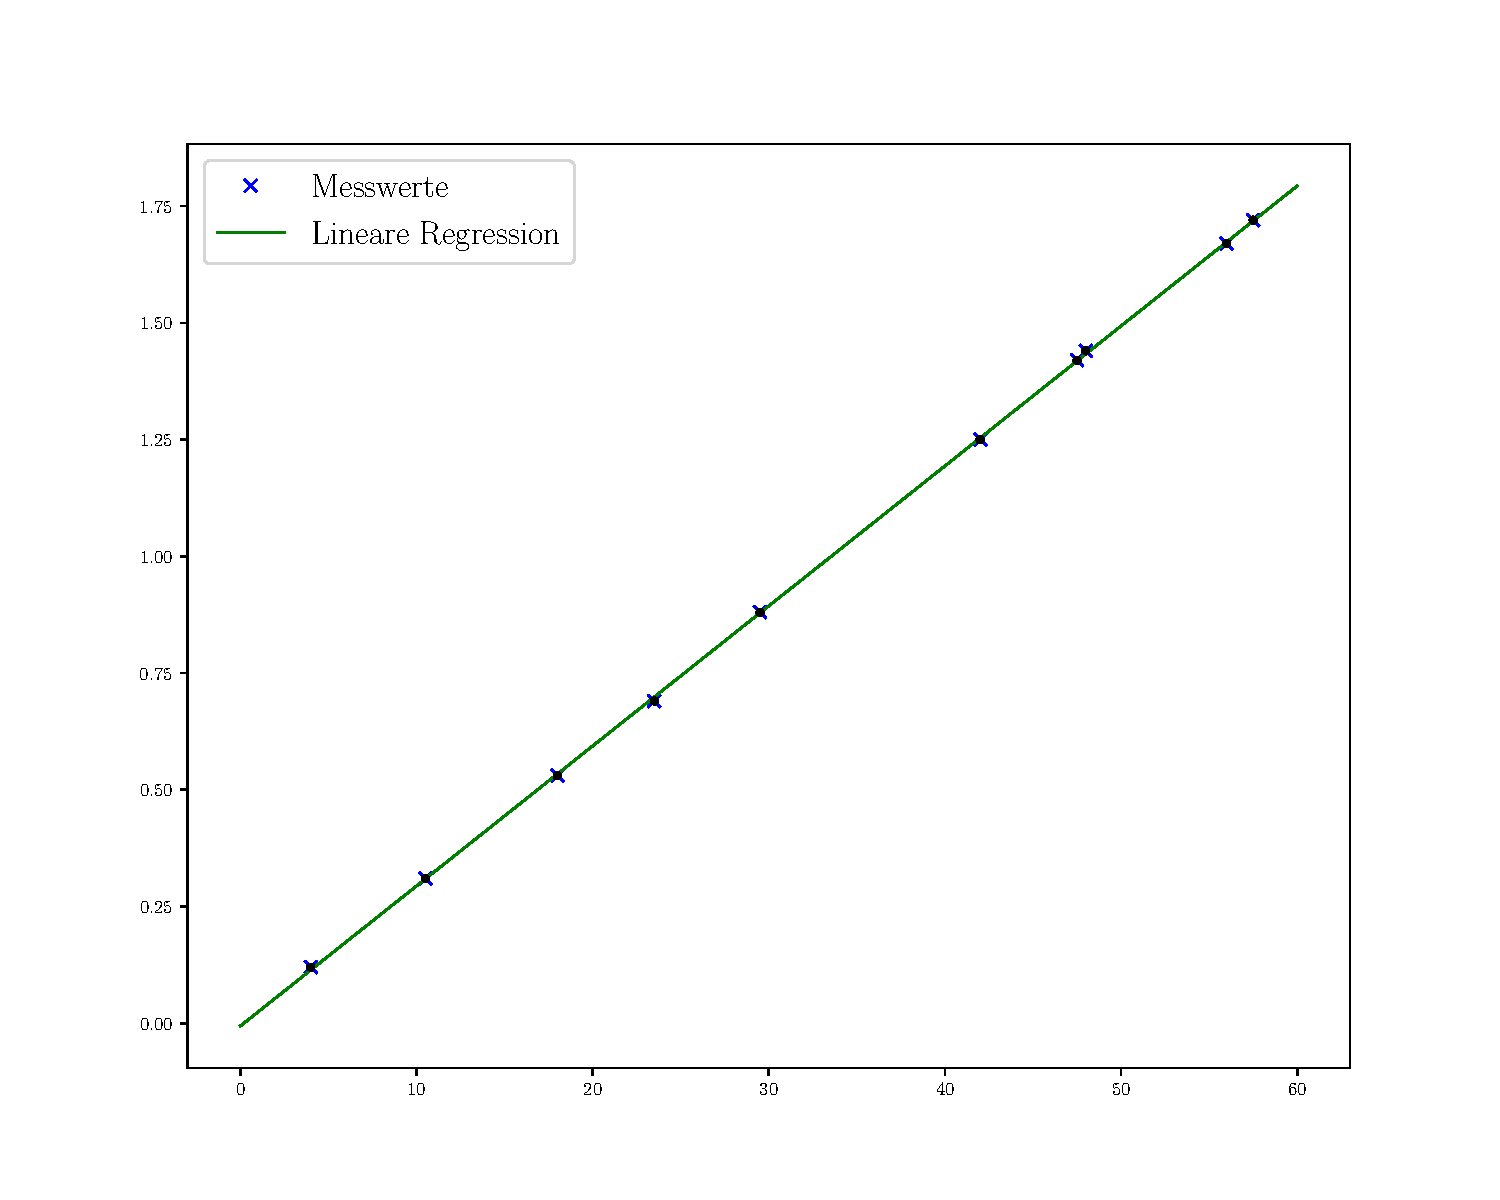
\includegraphics{Plot.pdf}
    \caption{Plot.}
    \label{fig:plot}
  \end{figure}
  
  
Die lineare Ausgleichsrechnung ist ersichtlich auf \autoref{fig:plot}.